% Ubah judul dan label berikut sesuai dengan yang diinginkan.
\section{Arsitektur}
\label{sec:arsitektur}

% Ubah paragraf-paragraf pada bagian ini sesuai dengan yang diinginkan.

\subsection{Dataset Penelitian}
\label{subsec:dataset}

Data yang digunakan dalam penelitian ini adalah data yang diperoleh dari Diabetic Retinopathy Analisis Grand challenge, berupa citra OCT-\emph{Angiography}.
Untuk persebaran data yang digunakan pada penelitian ini, terdapat pada tabel \ref{table:Datasettraining}

	\begin{figure}[hbtp]
		\centering
		\subfloat[\centering Non-DR]{{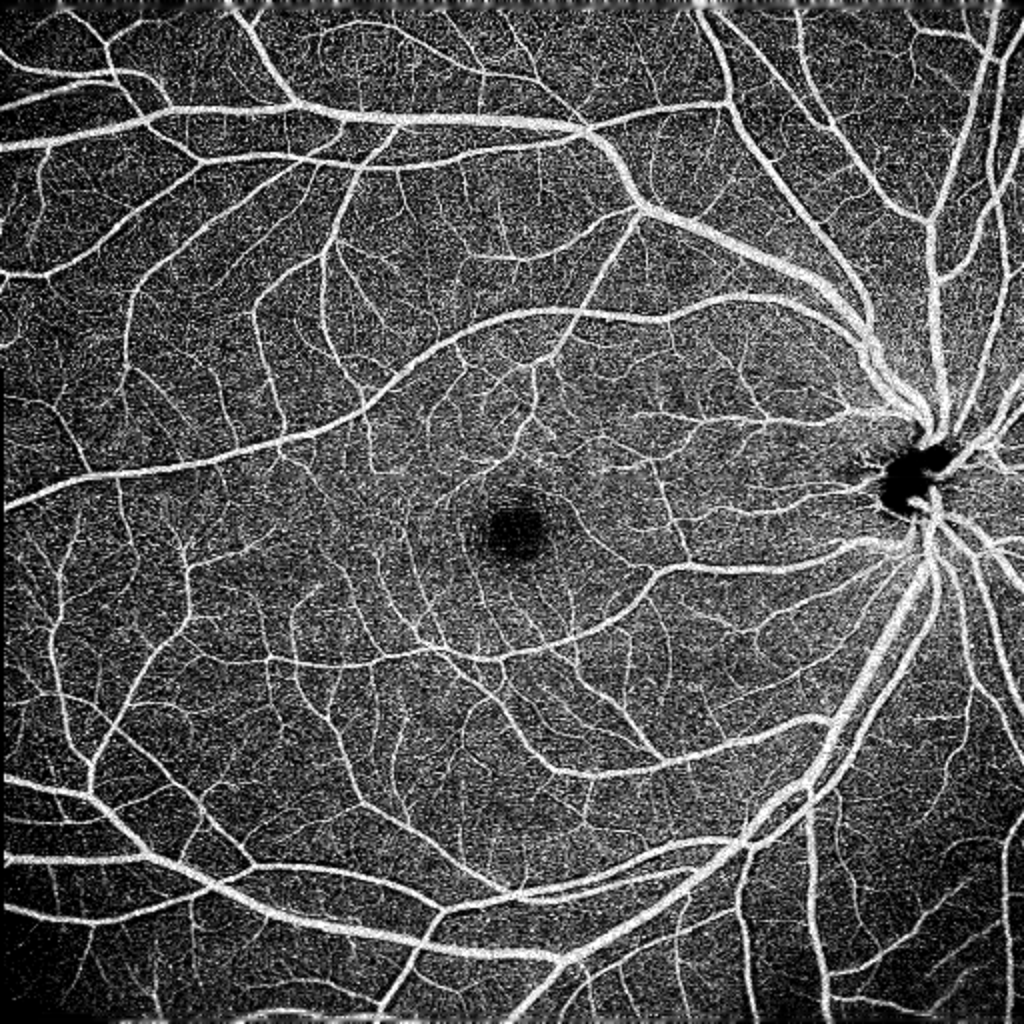
\includegraphics[width=2.5cm]{gambar/non-DR.png} }}%
		\subfloat[\centering NPDR]{{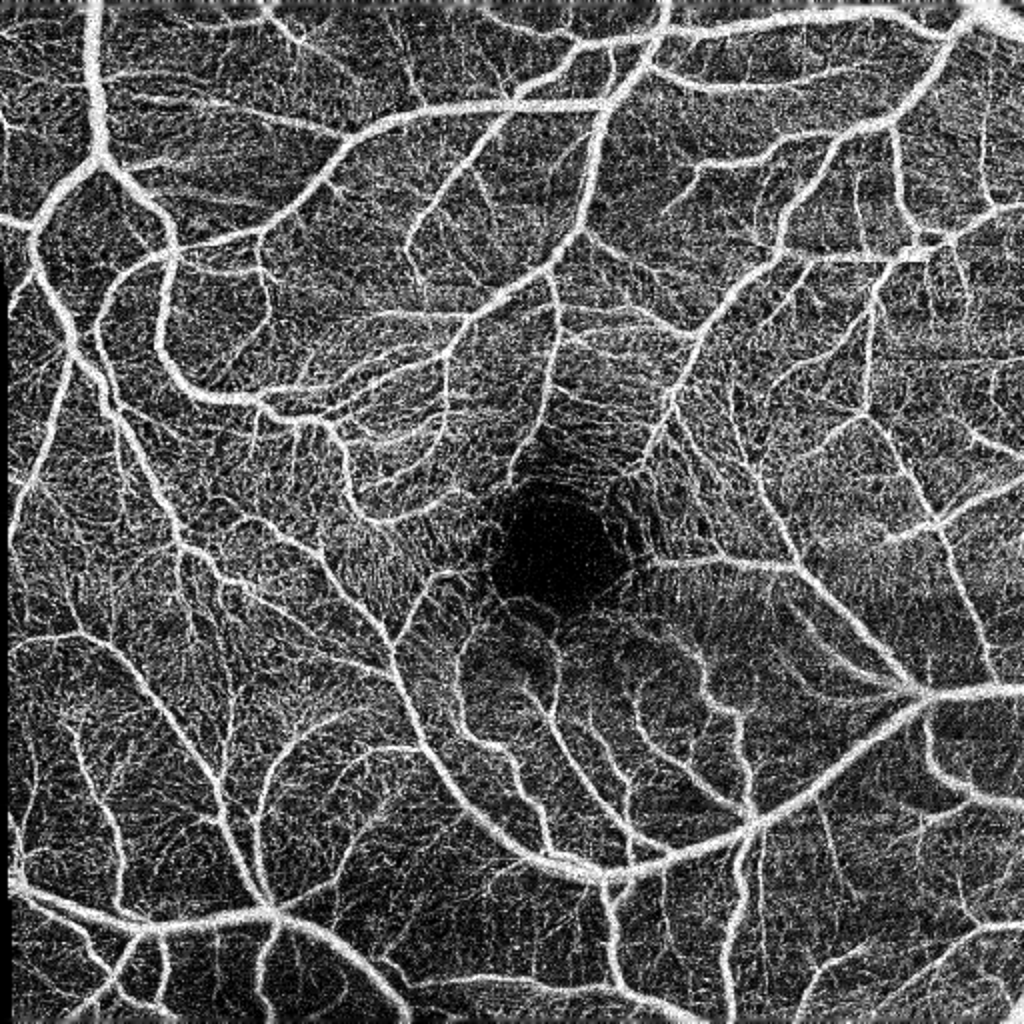
\includegraphics[width=2.5cm]{gambar/NPDR.png} }}%
		\subfloat[\centering PDR]{{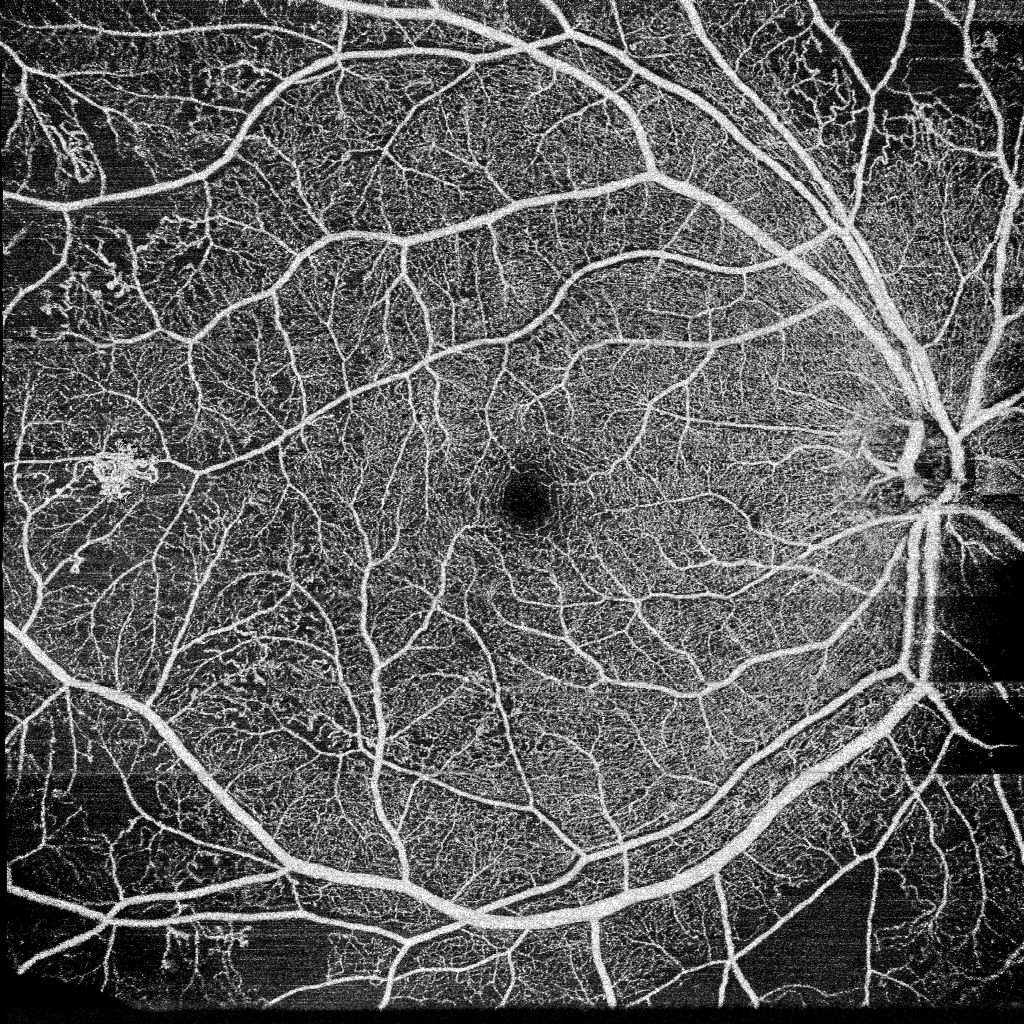
\includegraphics[width=2.5cm]{gambar/PDR.png} }}%
		\caption{Contoh Data Citra Retina}
		\label{fig:sampleDataset}
	\end{figure}
Gambar yang diberikan adalah foto fundus retina yang digunakan untuk evaluasi retinopati diabetik. Foto ini menunjukkan detail dari jaringan pembuluh darah retina, disk optik, dan area makula. Berikut adalah deskripsi rinci dari gambar tersebut:

Informasi Dataset dari Tantangan DRAC
Dataset yang digunakan untuk pelatihan dan pengujian terdiri dari:

	\begin{itemize}
		\item Set Pelatihan: 611 gambar
		\item Set Uji: 386 gambar
	\end{itemize}
Gambar-gambar pada set pelatihan, kemudian dipisah kembali menjadi dua set, yaitu set untuk pelatihan dan set untuk validasi dengan jumlah sesuai pada tabel \ref{table:Datasettraining}

%\begin{table}[hbtp]
%	\begin{center}
%	\caption{Tabel distribusi Set untuk Pelatihan dan Validasi}
%	\label{table:Datasettraining}
%	\begin{tabular}{|l|l|l|l|}
%		\hline
%		\rowcolor[HTML]{C0C0C0} 
%		Label                                                & Klasifikasi & Jumlah & Total                                         \\ \hline
%		\rowcolor[HTML]{FFFFFF} 
%		\cellcolor[HTML]{FFFFFF}                             & non-DR      & 263    & \cellcolor[HTML]{FFFFFF}                      \\ \cline{2-3}
%		\rowcolor[HTML]{FFFFFF} 
%		\cellcolor[HTML]{FFFFFF}                             & NPDR        & 169    & \cellcolor[HTML]{FFFFFF}                      \\ \cline{2-3}
%		\rowcolor[HTML]{FFFFFF} 
%		\multirow{-3}{*}{\cellcolor[HTML]{FFFFFF}Training}   & PDR         & 56     & \multirow{-3}{*}{\cellcolor[HTML]{FFFFFF}488} \\ \hline
%		\rowcolor[HTML]{FFFFFF} 
%		\cellcolor[HTML]{FFFFFF}                             & non-DR      & 66     & \cellcolor[HTML]{FFFFFF}                      \\ \cline{2-3}
%		\rowcolor[HTML]{FFFFFF} 
%		\cellcolor[HTML]{FFFFFF}                             & NPDR        & 43     & \cellcolor[HTML]{FFFFFF}                      \\ \cline{2-3}
%		\rowcolor[HTML]{FFFFFF} 
%		\multirow{-3}{*}{\cellcolor[HTML]{FFFFFF}Validation} & PDR         & 14     & \multirow{-3}{*}{\cellcolor[HTML]{FFFFFF}123} \\ \hline
%		\end{tabular}
%	\end{center}
%\end{table}

Sedangkan gambar pada set uji digunakan untuk mendapatkan penilaian online menggunakan metrik Quadratic Weighted Kappa dengan model dari DRAC sebagai pembandingnya. dan dikarenakan set uji yang diberikan ini tidak memiliki label, maka set ini tidak dapat dipergunakan untuk pengambilan metrik lain seperti \emph{precision, recall}, dan \emph{F1-score}.

\subsection{Methodology}
\label{subsec:loremipsum}

Perbandingan metode skenario yang digunakan dalam pelatihan model ResNet:
Dalam penelitian ini, dikarenakan oleh dataset yang sedikit dan ada class yang kurang representatif, dilakukan beberapa metode untuk penyeimbangan dataset.
\begin{itemize}
	\item Default
	
	Tidak ada Tindakan yang dilakukan untuk menyeimbangkan dataset. Metode ini dilakukan untuk variabel kontrol
	\item Penyesuaian \emph{Class-weight}
	
	Pada metode ini, dilakukan penambahan weight agar class yang underrepresented memiliki beban lebih tinggi
\end{itemize}

\begin{figure}[hbtp] \centering
	% Nama dari file gambar yang diinputkan
	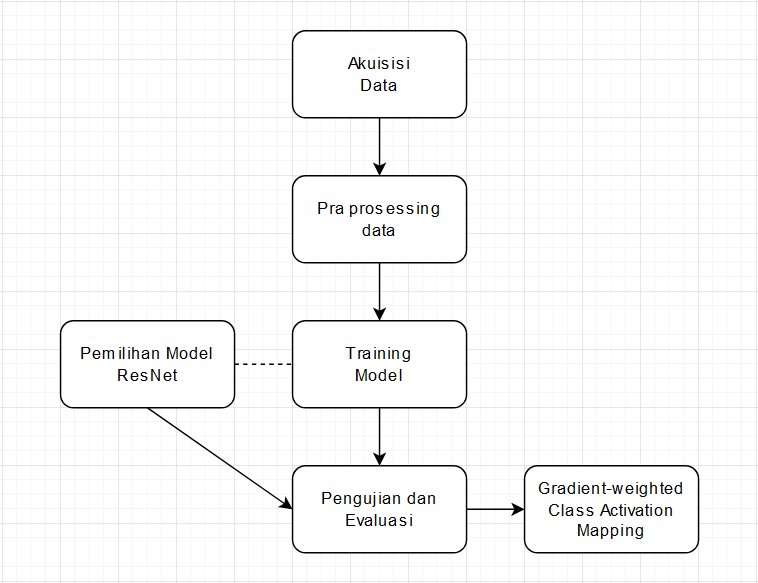
\includegraphics[scale=0.5]{gambar/diagramMethod.png}
	% Keterangan gambar yang diinputkan
	\caption{Diagram blok metodologi}
	% Label referensi dari gambar yang diinputkan
	\label{fig:diagramMethod}
\end{figure}

\subsection{Pelatihan Model}
\label{sec:325}
Pelatihan model dilakukan dengan menggunakan metode \emph{transfer learning}. Metode \emph{transfer learning} dilakukan dengan menggunakan model ResNet yang sudah dipilih dan sudah dilatih dengan dataset ImageNet.
Arsitektur model yang digunakan sesuai pada penjelasan bagian \ref{sec:323} dengan menggunakan \emph{hyper-parameter} yang ada pada tabel \ref{tb:hyperParameterTraining}
\begin{table}[hbtp]
	\begin{center}
		\caption{Hyperparameter}
		\label{tb:hyperParameterTraining}
		\begin{tabular}{|
		>{\columncolor[HTML]{C0C0C0}}l |l|lll}
		\cline{1-2}
		Input shape                                         & 224,224,3      &  &  &  \\ \cline{1-2}
		Opimizer                                            & Adam           &  &  &  \\ \cline{1-2}
		Loss Function                                       & Cross Entropy  &  &  &  \\ \cline{1-2}
		Learning Rate                                       & 0.1            &  &  &  \\ \cline{1-2}
		Momentum                                            & 0.9            &  &  &  \\ \cline{1-2}
		\cellcolor[HTML]{C0C0C0}                            & Step size = 10 &  &  &  \\ \cline{2-2}
		\multirow{-2}{*}{\cellcolor[HTML]{C0C0C0}Scheduler} & Gamma = 0.1    &  &  &  \\ \cline{1-2}
		Epoch                                               & 100            &  &  &  \\ \cline{1-2}
		Batch size                                          & 32             &  &  &  \\ \cline{1-2}
		\end{tabular}
	\end{center}
\end{table}


% Contoh pembuatan potongan kode.
%\begin{lstlisting}[
%  language=C++,
%  caption={Program halo dunia.},
%  label={lst:halodunia}
%]
%#include <iostream>
%
%int main() {
%    std::cout << "Halo Dunia!";
%    return 0;
%}
%\end{lstlisting}